\subsubsection{Venue : Creating new venue}
	Once a user has been successfully authenticated by the UPRM system, the user should be able to create a new venue.\\ 
	The venue creation will require the following information before the creation is finalised: 
	\begin{itemize}
		\item Name of the new venue.
		\item The name of the organisation responsible for the venue.
		\item A date signifying the deadline for submissions.
		\item Contact details to where the submissions should be posted (i.e. email address).\\
	\end{itemize}
	\textbf{Pre-Conditions}
	\begin{itemize}
		\item User has to be successfully authenticated.\\
	\end{itemize}
	\textbf{Post-Conditions}
	\begin{itemize}
		\item A new venue should be created.
		\item The new venue information should be saved in a database.\\
	\end{itemize}
	\textbf{Use case diagram for creation of venues: }\\
	\centerline{\fbox{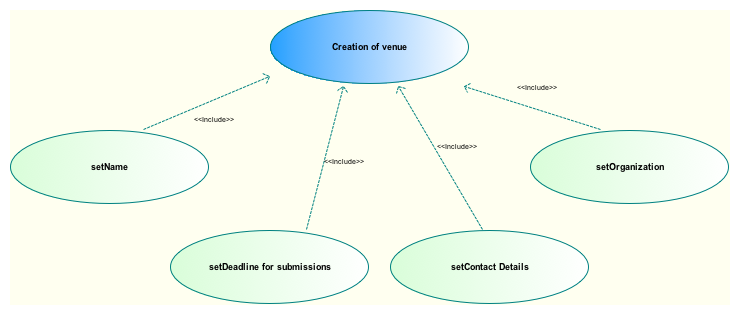
\includegraphics[width=\linewidth]{venue/uprm_venueCreate.png}}}
	
\subsubsection{Venue : Updating venue}
If a venue exists and the authenticated user wishes to change some information regarding their venue then the user should be able to do so. \\ \\
The user should be able to change the following information of a venue: 
\begin{itemize}
	\item Name of the venue.
	\item The date signifying the deadline for submissions.
	\item Contact details to where the submissions should be posted (i.e. email address).\\ \\
\end{itemize}
\textbf{Pre-Conditions}
\begin{itemize}
	\item User has to be successfully authenticated.
	\item The venue should already exist.\\
\end{itemize}
\textbf{Post-Conditions}
\begin{itemize}
	\item A venue should be updated.
	\item The venue information should be updated in a database.\\
\end{itemize}
\textbf{Use case diagram for updating of venues: }\\
\centerline{\fbox{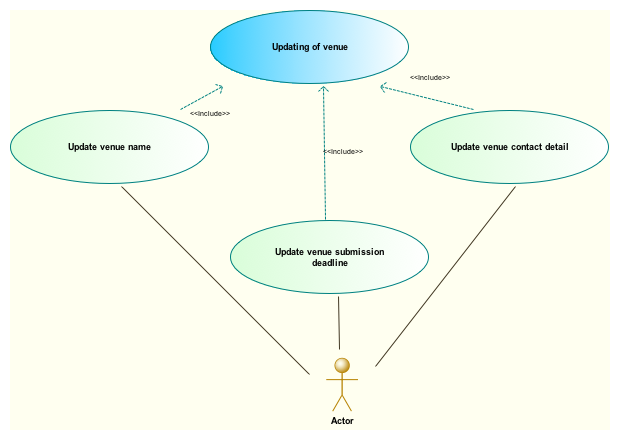
\includegraphics[width=\linewidth]{venue/uprm_venueUpdate.png}}}

\subsubsection{Venue : Deleting venue}
If a venue exists and the authenticated user wishes to remove a venue from the UPRM system. \\ \\
\textbf{Pre-Conditions}
\begin{itemize}
	\item User has to be successfully authenticated.
	\item The venue should already exist.
	\item There should not be any pending submissions.\\
\end{itemize}
\textbf{Post-Conditions}
\begin{itemize}
	\item The venue should be completely removed from the UPRM database.\\
\end{itemize}

\subsubsection{Venue : Sending feedback and updating status}
Once a submission is received and has been reviewed by the venue, the venue can send feedback to the project.\\ \\
\textbf{Pre-Conditions}
\begin{itemize}
	\item User has to be successfully authenticated.
	\item The venue should already exist.
	\item The project should already exist.\\
\end{itemize}
\textbf{Post-Conditions}
\begin{itemize}
	\item The project feedback information should be updated in the database and a notification sent out.
	\item The status of the project should change.\\
\end{itemize}